La résolution du problème via Matlab nous montre que, lorsque le nombre d'ouvriers est constant, l'usine tourne à plein régime en permanence, accumule beaucoup de stock et de retard, jusqu'à parfois devoir recourir à la sous-traitance pour livrer dans les temps.

Il semble évident qu'un important bottleneck se situe au niveau du nombre d'ouviers disponibles, d'où l'ajout, à partir de la question 7, du nombre variable d'ouviers.

\begin{figure}[h]
    \centering
    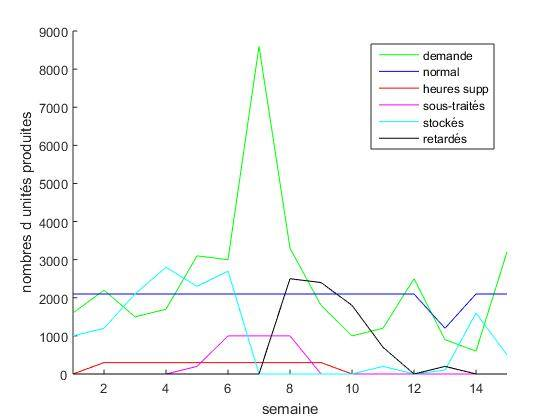
\includegraphics[width=0.8\textwidth]{graphes/q3.jpg}
    \caption{Graphe de la production à personnel constant}
    \label{fig:q3}
\end{figure}
%TODO: graphe
